\section{Performances des supercalculateurs}\label{sec:edl_evolution}
%%%%%%%%%%%%%%%%%%%%%%%%%%%%%%%%%%%%%%%%%%%%%%%%%%%%%%%%%%%





\subsection{Comparer la performance des supercalculateur}
%%%%%%%%%%%%%%%%%%%%%%%%%%%%%%%%%%%%%%%%%%%%%
        
        Pour comparer la performance des supercalculateurs, un code de référence doit être utilisé. Le benchmarking ou l'étalonnage est une pratique courante qui consiste à évaluer plusieurs solutions en leur faisant passer un épreuve commune. Dans le domaine informatique cela permet de tester différentes architectures matériels et d'évaluer leurs performances. Il existe plusieurs benchmark qui ont chacune leur particularités. Le benchmark le plus populaire dans le domaine du HPC est celui développé par Jack Dongara en 1988: le benchmark HPL \cite{Dongarra}. C'est grâce à lui que le classement du TOP500 est réalisé deux fois par ans. Ce benchmark est un code simple qui résout un système d'équation linéaire de deux matrices $A$ et $B$ par $Ax = B$. L'avantage de ce code est que les performances évoluent linéairement avec le nombre de machines utilisées car il y a très peu de communication sur le réseaux. Le résultat est un nombre de FLOP/S que la machine peut exécuter, ce qui rend la comparaison avec d'autres supercalculateur facile. 
    
    
        Ce code permet de réaliser deux classements biannuels: le Top500 et le Green500 (\autoref{fig:Top500}). Le Green500 classe les 500 supercalculateurs les plus énergétiquement efficaces parmi les supercalculateurs classés dans le TOP500.
        
        \begin{figure}[t!]
                \centering
                \begin{subfigure}[t]{0.48\textwidth}
                    \centering
                    
\includegraphics[width=.4\linewidth]{images/Top500_logo.png}
                    \caption{\label{fig:Top500_logo}Top500}
                \end{subfigure}\hfill
            \begin{subfigure}[t]{0.48\textwidth}
                    \centering
                    
\includegraphics[width=.25\linewidth]{images/Green500_logo.png}
                    \caption{\label{fig:Green500_logo}Green500}
            \end{subfigure}
            \caption{\label{fig:Top500} Les classements du Top500 et du Green500 sont présentés deux fois par an lors de la conférence Supercomputing\protect\footnotemark}
        \end{figure}
        \footnotetext{\url{supercomputing.org/}}
        
    
    \subsubsection{Le Top500}
    %%%%%%%%%%%%%%%%%%%%%%%%%%%%%%%%%%%%%%%%%%%%%
        
        Le TOP500\footnote{\url{www.top500.org}} est un classement mondial qui classe, tous les 6 mois depuis 1993, les 500 super-calculateurs les plus puissants au monde. Ce classement se base sur le nombre maximum d'opérations flottantes qui peuvent être exécutées en une secondes. Cette unité à été choisie car la grande majorité des codes utilisés dans les domaines précédemment cités, exécutent des opérations sur des nombres flottant. Il s'avère donc judicieux de choisir ce dénominateur commun pour comparer les différentes architectures.
        
        Il faut cependant savoir que ce classement ne contient pas toutes les machines. En effet, certains industriels ne préfèrent pas paraître dans ce classement. Stratégiquement parlant, il peut être intéressant de ne pas publier sa puissance de calcul et nous savons que les clusters les plus puissants n'y figurent pas. Cependant ce classement nous permet de voir les tendances que suivent la majorité des architectures pour comprendre comment elles évoluent.
   
        Au moment de l'écriture de ce manuscrit, le dernier classement disponible est celui de novembre 2019\footnote{\url{www.top500.org/lists/2019/11/}}. Les principales caractéristiques des quatres premiers supercalculateurs sont présentées dans le \autoref{tab:top500}. Les États-Unis et la Chine possèdent chacun deux entrées et se partagent 70\% des performances totales du Top500 (32.3\% pour la Chine, 37.1\% pour les États-Unis).
        Les deux supercalculateurs les plus puissants sont construit par AMD et utilisent chacun des accélérateurs GPU Nvidia Tesla V100.
        L'efficacité des supercalculateurs représente la capacité d'une plateforme à atteindre la performances théoriques \verb|Rpeak|. Sur les 500 plateformes répertoriées, 100 d'entre elles ne parviennent pas à atteindre plus de 50\% de la performance théorique. Cette informations est importante pour comprendre la difficulté des applications à utiliser ces plateformes efficacement. Le benchmark \verb|HPL| est un code très simple, avec peu d'accès mémoire. Les applications réelles, plus complexes, ont beaucoup de mal à atteindre cette efficacité. Depuis quelques années, le classement du Top500 donne la performance d'un second benchmark (HPCG, voir \autoref{sec:hpcg}). Pour ce benchmark, plus fidèle aux comportements d'applications réelles, aucune des plateformes n'atteint une efficacité supérieur à 4\%.
        Concernant le système d'interconnexion, 6 des 10 premieres entrées utilisent la technologie Infiniband, ainsi que 141 des 500 supercalculateurs.
        La consommation électrique de ces quatre plateformes varie de 7 à 18 mégawatt. On remarque que le premier supercalculateur du classement n'est pas celui consommant le plus d'énergie. Pour avoir une meilleure vision de l'efficacité des plateformes, le classement du Green500 peut être consulté.

        \begin{table}[]
\centering
\resizebox{\textwidth}{!}{%
\begin{tabular}{|c|c|c|r|r|r|c|r|r|r|}
\hline
\rowcolor[HTML]{EFEFEF} 
\textbf{Pos.} & \textbf{Nom} & \multicolumn{1}{l|}{\cellcolor[HTML]{EFEFEF}\textbf{Country}} & \multicolumn{1}{l|}{\cellcolor[HTML]{EFEFEF}\textbf{Nb. coeurs}} & \multicolumn{1}{l|}{\cellcolor[HTML]{EFEFEF}\textbf{Coeurs accélérateur}} & \multicolumn{1}{l|}{\cellcolor[HTML]{EFEFEF}\textbf{Alimentation (MW)}} & \multicolumn{1}{l|}{\cellcolor[HTML]{EFEFEF}\textbf{Accélérateur}} & \multicolumn{1}{c|}{\cellcolor[HTML]{EFEFEF}\textbf{Rpeak}} & \multicolumn{1}{c|}{\cellcolor[HTML]{EFEFEF}\textbf{Rmax}} & \multicolumn{1}{c|}{\cellcolor[HTML]{EFEFEF}\textbf{Éfficacité}} \\ \hline
1 & Summit & United States & 2414592 & 2211840 & 10 & NVIDIA GPU & 200 & 148 & 0.74 \\ \hline
2 & Sierra & United States & 1572480 & 1382400 & 7 & NVIDIA GPU & 125 & 94 & 0.75 \\ \hline
3 & Sunway TaihuLight & China & 10649600 & 0 & 15 & None & 125 & 93 & 0.74 \\ \hline
4 & Tianhe-2A & China & 4981760 & 4554752 & 18 & Matrix-2000 & 100 & 61 & 0.61 \\ \hline
\end{tabular}%
}
\caption{Classement du Top500 de novembre 2019. Les puissances Rpeak (puissance théorique) et Rmax (puissance mesurée par HPL) sont données en PFlops ($10^{15}$ flops)}
\label{tab:top500}
\end{table}
   
   
    
    \subsubsection{Le Green500}
    %%%%%%%%%%%%%%%%%%%%%%%%%%%%%
    
        Ces vingt dernières années, les évolutions technologiques et l'augmentation de la taille des supercalculateurs n'avait pas de limite physique. Cette course à la performance n'était dictée que par les budget disponibles pour leur construction. Ainsi, nous avons constaté l'émergence de plateformes consommant de grande quantités d'énergie et très peu efficace (voir le classement du Top500). 
        
        Un second classement à donc vu le jour en 2007 appelé le Green500\footnote{\url{www.top500.org/green500/}}. Il classe les supercalculateurs selon un critère d’efficacité énergétique. Cette efficacité mesure le nombre d’opérations sur un nombre flottant réalisé pour 1 watt d’énergie prodigué au supercalculateur. 
        
        En novembre 2019\footnote{\url{www.top500.org/green500/lists/2019/11/}}, les 34 premiers supercalculateurs utilisent tous des accélérateurs. La majorité étant des GPU Nvidia Tesla. Il est intéressant de noter que la deuxième place du classement est tenu par une plateforme basée sur le processeur PEZY-SC2 conçu par TSMC. Seul le premier du classement n'utilise pas d'accélérateurs (voir \autoref{tab:green500}). Il utilise un processeur ARM basse fréquence pouvante exécuter des instructions vectorielles SVE (Scalable Vector Extensions) sur 512 bits.
        
        \begin{table}[]
\centering
\resizebox{0.80\textwidth}{!}{%
\begin{tabular}{|c|r|l|l|r|r|r|r|}
\hline
\rowcolor[HTML]{EFEFEF} 
\textbf{Position} & \multicolumn{1}{c|}{\cellcolor[HTML]{EFEFEF}\textbf{TOP500}} & \multicolumn{1}{c|}{\cellcolor[HTML]{EFEFEF}\textbf{Processeur}} & \multicolumn{1}{c|}{\cellcolor[HTML]{EFEFEF}\textbf{Accélérateur}} & \multicolumn{1}{c|}{\cellcolor[HTML]{EFEFEF}\textbf{Rmax}} & \multicolumn{1}{c|}{\cellcolor[HTML]{EFEFEF}\textbf{Rpeak}} & \multicolumn{1}{c|}{\cellcolor[HTML]{EFEFEF}\textbf{Efficacité}} & \multicolumn{1}{c|}{\cellcolor[HTML]{EFEFEF}\textbf{Efficacité énergétique}} \\ \hline
1 & 159 & Fujitsu A64FX & Aucun & 1.99 & 2.35 & 0.84 & 16.876 \\ \hline
2 & 420 & Xeon D-1571 & PEZY-SC2 700Mhz & 1.30 & 1.79 & 0.72 & 16.256 \\ \hline
3 & 24 & IBM POWER9 & Volta GV100 & 8.04 & 11.12 & 0.72 & 15.771 \\ \hline
4 & 373 & IBM POWER9 & Tesla V100 SXM2 & 1.46 & 1.73 & 0.84 & 15.574 \\ \hline
\end{tabular}%
}
\caption{Classement du Green500 de novembre 2019 selon l'efficacité énergétique (en GFlops/Watts). Les puissances Rpeak (puissance théorique) et Rmax (puissance mesurée par HPL) sont données en PFlops ($10^{15}$ flops).}
\label{tab:green500}
\end{table}
        
        

        
   
\subsection{Évolution des performances des supercalculateurs}
%%%%%%%%%%%%%%%%%%%%%%%%%%%%%%%%%%%%%%

    Le classement du Top500 à de nombreux avantages, dont celui de promouvoir le HPC au grand public. Cependant, un effet de bord de ce classement est de motiver les constructeurs pour développer des architectures ayant de bonnes performances lors de l'exécution du benchmark HPC. Or, ce code n'est pas représentatif des applications réelles et nous pouvons nous demander si son utilisation pour l'établissement du Top500 n'a pas été contre productif. Bien que certains des supercalculateurs les plus puissant n'y figurent pas, l'évolution du Top500 permet d'obtenir un aperçu des évolutions de performances des architectures.
    
    
    Pour avoir une vision globale de son évolution, nous étudions la performances cumulées des 500 supercalculateurs depuis le premier classement (voir \autoref{pic_top500perf_evo}). Nous distinguons deux phases: avant et après 2012. 
    Avant 2012, la puissance des supercalculateurs a été multiplié par 1000 tout les 11 ans. Après 2012, il faut attendre 23 ans pour voir leur puissance évoluer du même facteur. 
    
    Dans cette section, nous discutons des différents facteurs qui ont permis l'évolution constante des performances des architectures pendant près de 20 ans et quels sont les freins qui empêchent de poursuivre ce rythme. La majorité des améliorations évoquées ont été présenté dans le \autoref{chap:sota:materiel}.
    
    \begin{figure}
        \center
        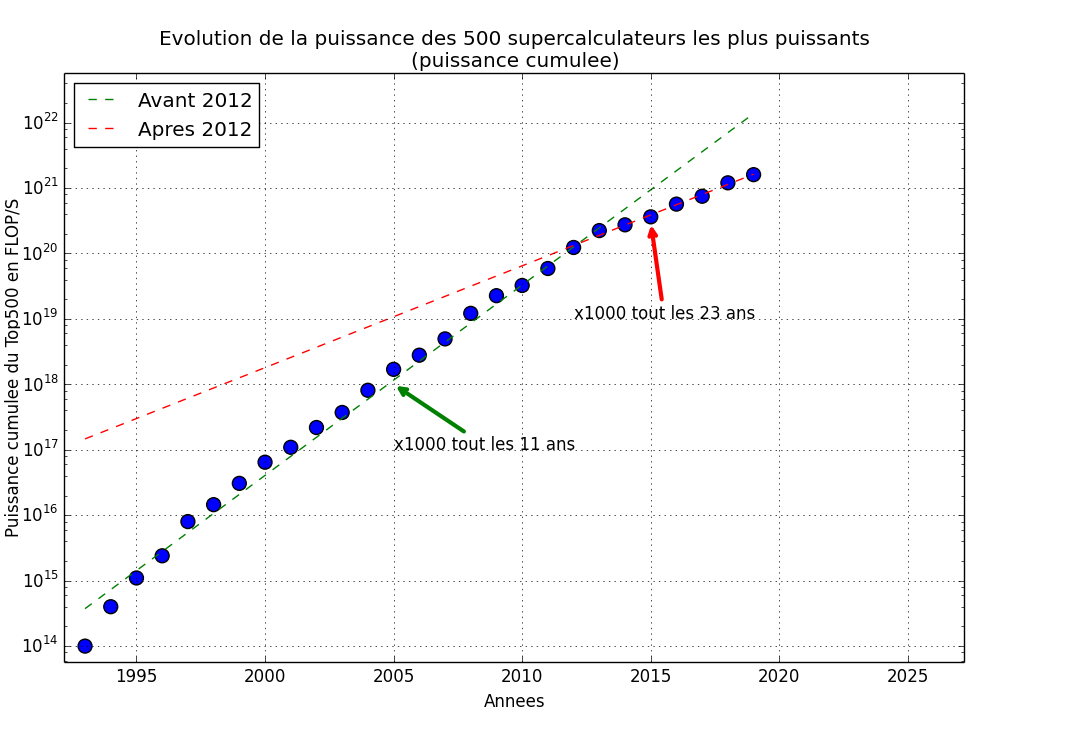
\includegraphics[width=10cm]{images/top500_evolution.png}
        \caption{\label{pic_top500perf_evo} Évolution de la performance cumulée des 500 supercalculateurs les plus puissants au monde. La pente de l'évolution diminue à partir de 2012}
    \end{figure}


    \subsubsection{Avant 2012}
    %%%%%%%%%%%%%%%%%%%%%%%%%%%%
    
        Les supercalculateurs ont pû bénéficier de nouvelles technologiques ainsi que de nombreuses innovations techniques.
        
        \begin{figure}[t!]
            \centering
            \begin{subfigure}[t]{0.33\textwidth}
                \centering
                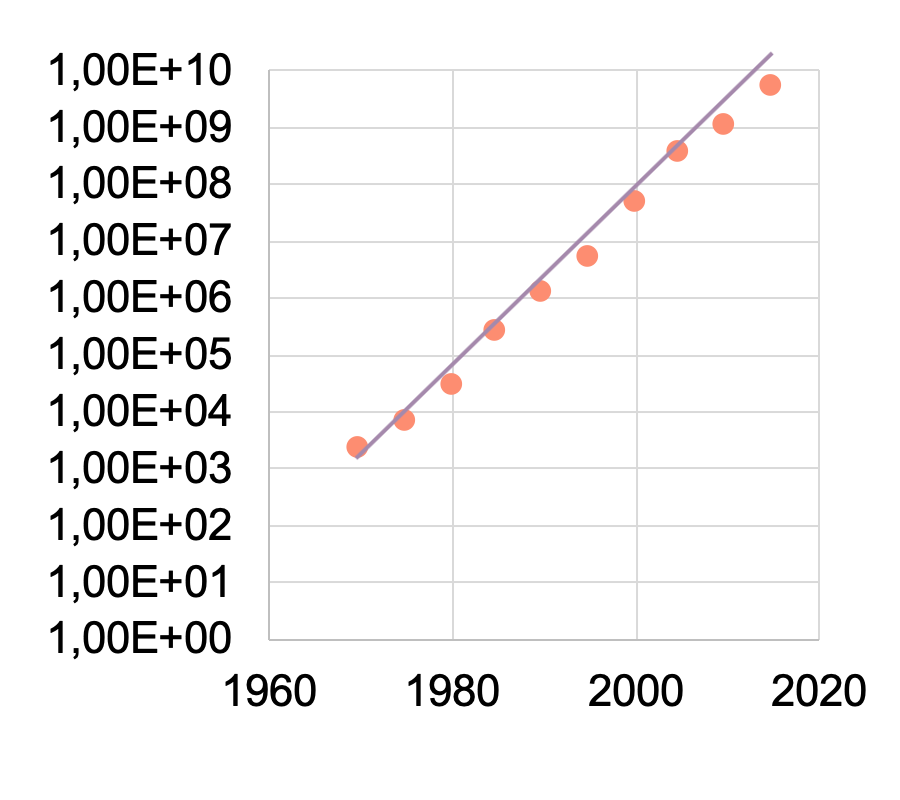
\includegraphics[width=\linewidth]{images/evo_transistor.png}
                \caption{\label{fig:evo_transistor}Évolution du nombre de transistors (voir \autoref{sec:denard})}
            \end{subfigure}\hfill
            \begin{subfigure}[t]{0.33\textwidth}
                \centering
                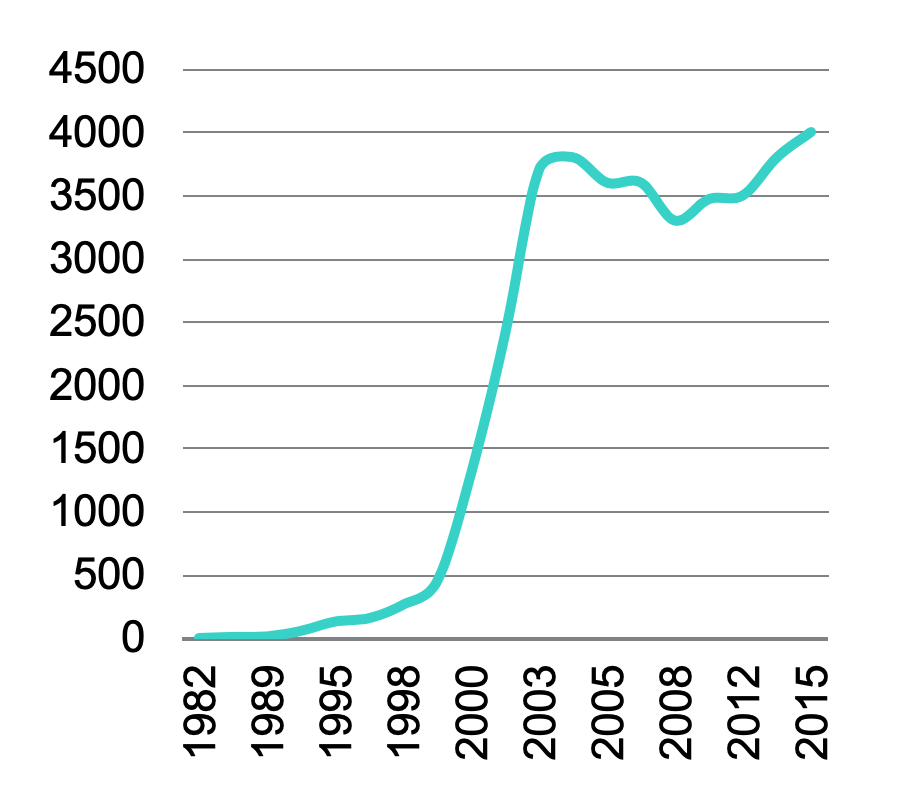
\includegraphics[width=\linewidth]{images/evo_freq.png}
                \caption{\label{fig:evo_freq}Évolution de la fréquence(voir \autoref{sec:frequency}}
            \end{subfigure}\hfill
            \begin{subfigure}[t]{0.33\textwidth}
                    \centering
                    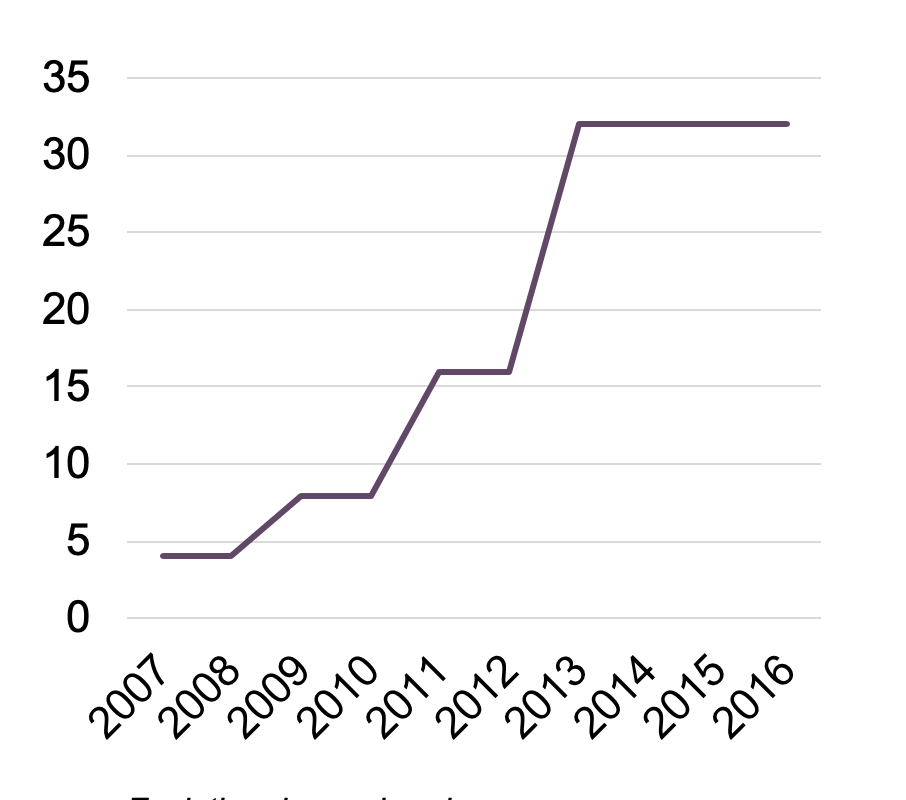
\includegraphics[width=\linewidth]{images/evo_core.png}
                    \caption{\label{fig:evo_core}Évolution du nombre de coeur (voir \autoref{sec:multicore})}
            \end{subfigure}
            \caption{\label{fig:evo_proc}Évolution technologiques principales des processeurs}
        \end{figure}
        
        \paragraph{Les processeurs.} Dans la \autoref{chap:sota:materiel}, nous avons présenté les différentes évolutions technologiques dont ont pu bénéficier les processeurs. La \autoref{fig:evo_proc} résume les trois principales évolutions.
        Grâce à l'affinement des procédés de gravure, le nombre de transistors à évolué exponentiellement (voir \autoref{fig:evo_transistor}).  
        En affinant les transistors et en utilisant des système de refroidissement plus efficaces, la fréquence des processeurs à pu être augmenté de plusieurs facteurs (voir \autoref{fig:evo_freq}).
        Lorsque la fréquence n'a plus pu être augmentée, les architectures parallèle ont été développé, donnant naissance au processeur multi-coeurs (voir \autoref{fig:evo_core}). La microarchitecture elle même à reçu de nombreuses améliorations: l'utilisation de pipeline (voir \autoref{sec:pipeline}) pouvant être superscalaire (voir \autoref{sec:superscalar}), ainsi que le développement d'unité de calculs pouvant exécuter des instructions vectoriels (voir \autoref{sec:cpu_vectoriel}).
            
    
        \paragraph{Les mémoires.} La performance des processeurs évoluant, celles des mémoires a aussi dû être améliorer pour fournir les données nécessaire aux traitements plus rapidement. Les principales amélioration sont dues à l'utilisation de nouvelles technologies mémoire (voir \autoref{sec:memory}), l'augmentation du nombre de canaux reliant la mémoire au processeur ou encore l'implémentation d'une hiérarchie de mémoire (voir \autoref{sec:hierarchie_true}). Celle-ci permettant aux applications de profiter du principe de localité (voir \autoref{sec:locality}).
        
            
    
    \subsubsection{Après 2012}
    %%%%%%%%%%%%%%%%%%%%%%%%%%%%
    
        En étudiant l'évolution de la puissance des supercalculateurs (voir \autoref{pic_top500perf_evo}), nous remarquons un ralentissement à partir des années 2010-2012. Ce ralentissement n’est pas dû à un seul facteur mais à un ensemble de contraintes. En effet, les leviers et évolutions technologiques qui permettaient de tenir cette cadence ne sont plus disponible aujourd’hui ou sont en fin de course.(voir \autoref{fig:evo_proc}). Il est intéressant de noter que tous les vecteurs qui ont permis aux performances d'évoluer ces 30 dernières années s'essoufflent simultanément. 
       
        \begin{figure}
            \center
            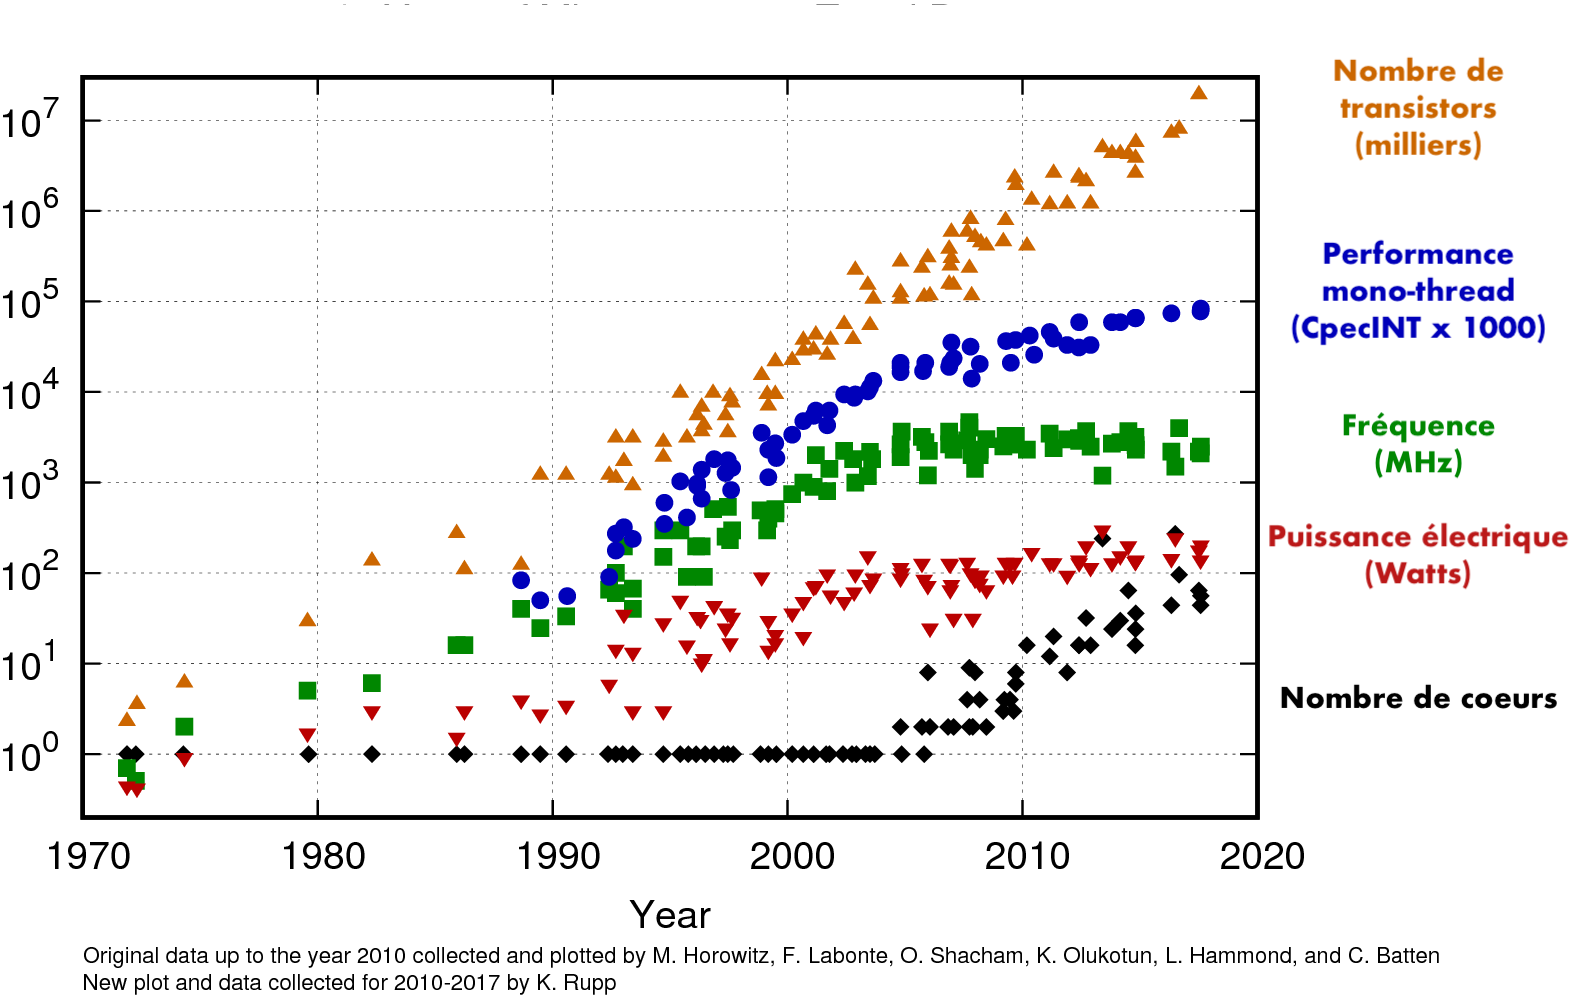
\includegraphics[width=12cm]{images/evo_proc.png}
            \caption{\label{fig:evo_proc} Évolution des principales caractéristiques des processeurs (données originales tirées de \cite{rupp40years}\protect\footnotemark).}
        \end{figure}
        \footnotetext{Les données sont accessibles sur le dépot GitHub de l'auter:  \url{https://github.com/karlrupp/microprocessor-trend-data}}
        
        %%%%%%%%%%%%%%%%%%%%%%%%%%%%%%%%%%%%%%%%%%%%%%%%%%%%%%%%%%%%%%%%%%%%%%%%%%%% 
        \paragraph{La fin des lois.} Si certaines lois ont assurer une évolution continue de la performance des processeurs pendant plusieurs dizaines d'années, celles-ci ont atteinte leur limite. Une partie du ralentissement de l'évolution des performances du Top500 peut être expliquée par leur \textit{essoufflement} \cite{FrancoisBodin2015}.
            
                
                \textbf{La loi de Moore} \cite{Moore1998}) prévoyait que les architectures pourrait doubler leur nombre de transistors à coût constant (voir \autoref{sec:moore}). Bien qu'elle ait été reformulée en 1975 \cite{Moore75}, les fondeurs ne parviennent plus à suivre le rythme dictée par la loi énoncée par Gordon Moore, pour des raisons principalement techniques (gravure), de coût \cite{Brooks2017} et de limite physique. À force de la réduire, les transistors ne mesurent plus que quelques nanomètres et à cette taille les courants électriques sont instables. Ne pouvant plus garantir la bonne circulation des signaux électrique dans les circuits, il n’est alors plus possible de réduire leur taille.
                À partir de 2013, l'évolution des performances du Top500 passe pour la première fois sous les performances prévues par la loi de Moore (\autoref{fig:moore_vs_top500}). Les performances du Top500 évoluées d'un facteur 1000 tous les 11 ans, profitant de la loi de Moore ainsi que des autres évolutions technologies présenté précédemment. À partir de 2013, il faut attendre en moyenne 20 ans pour voir la performances des supercalculateurs évoluer du même facteur.
                
                \begin{figure}
                \center
                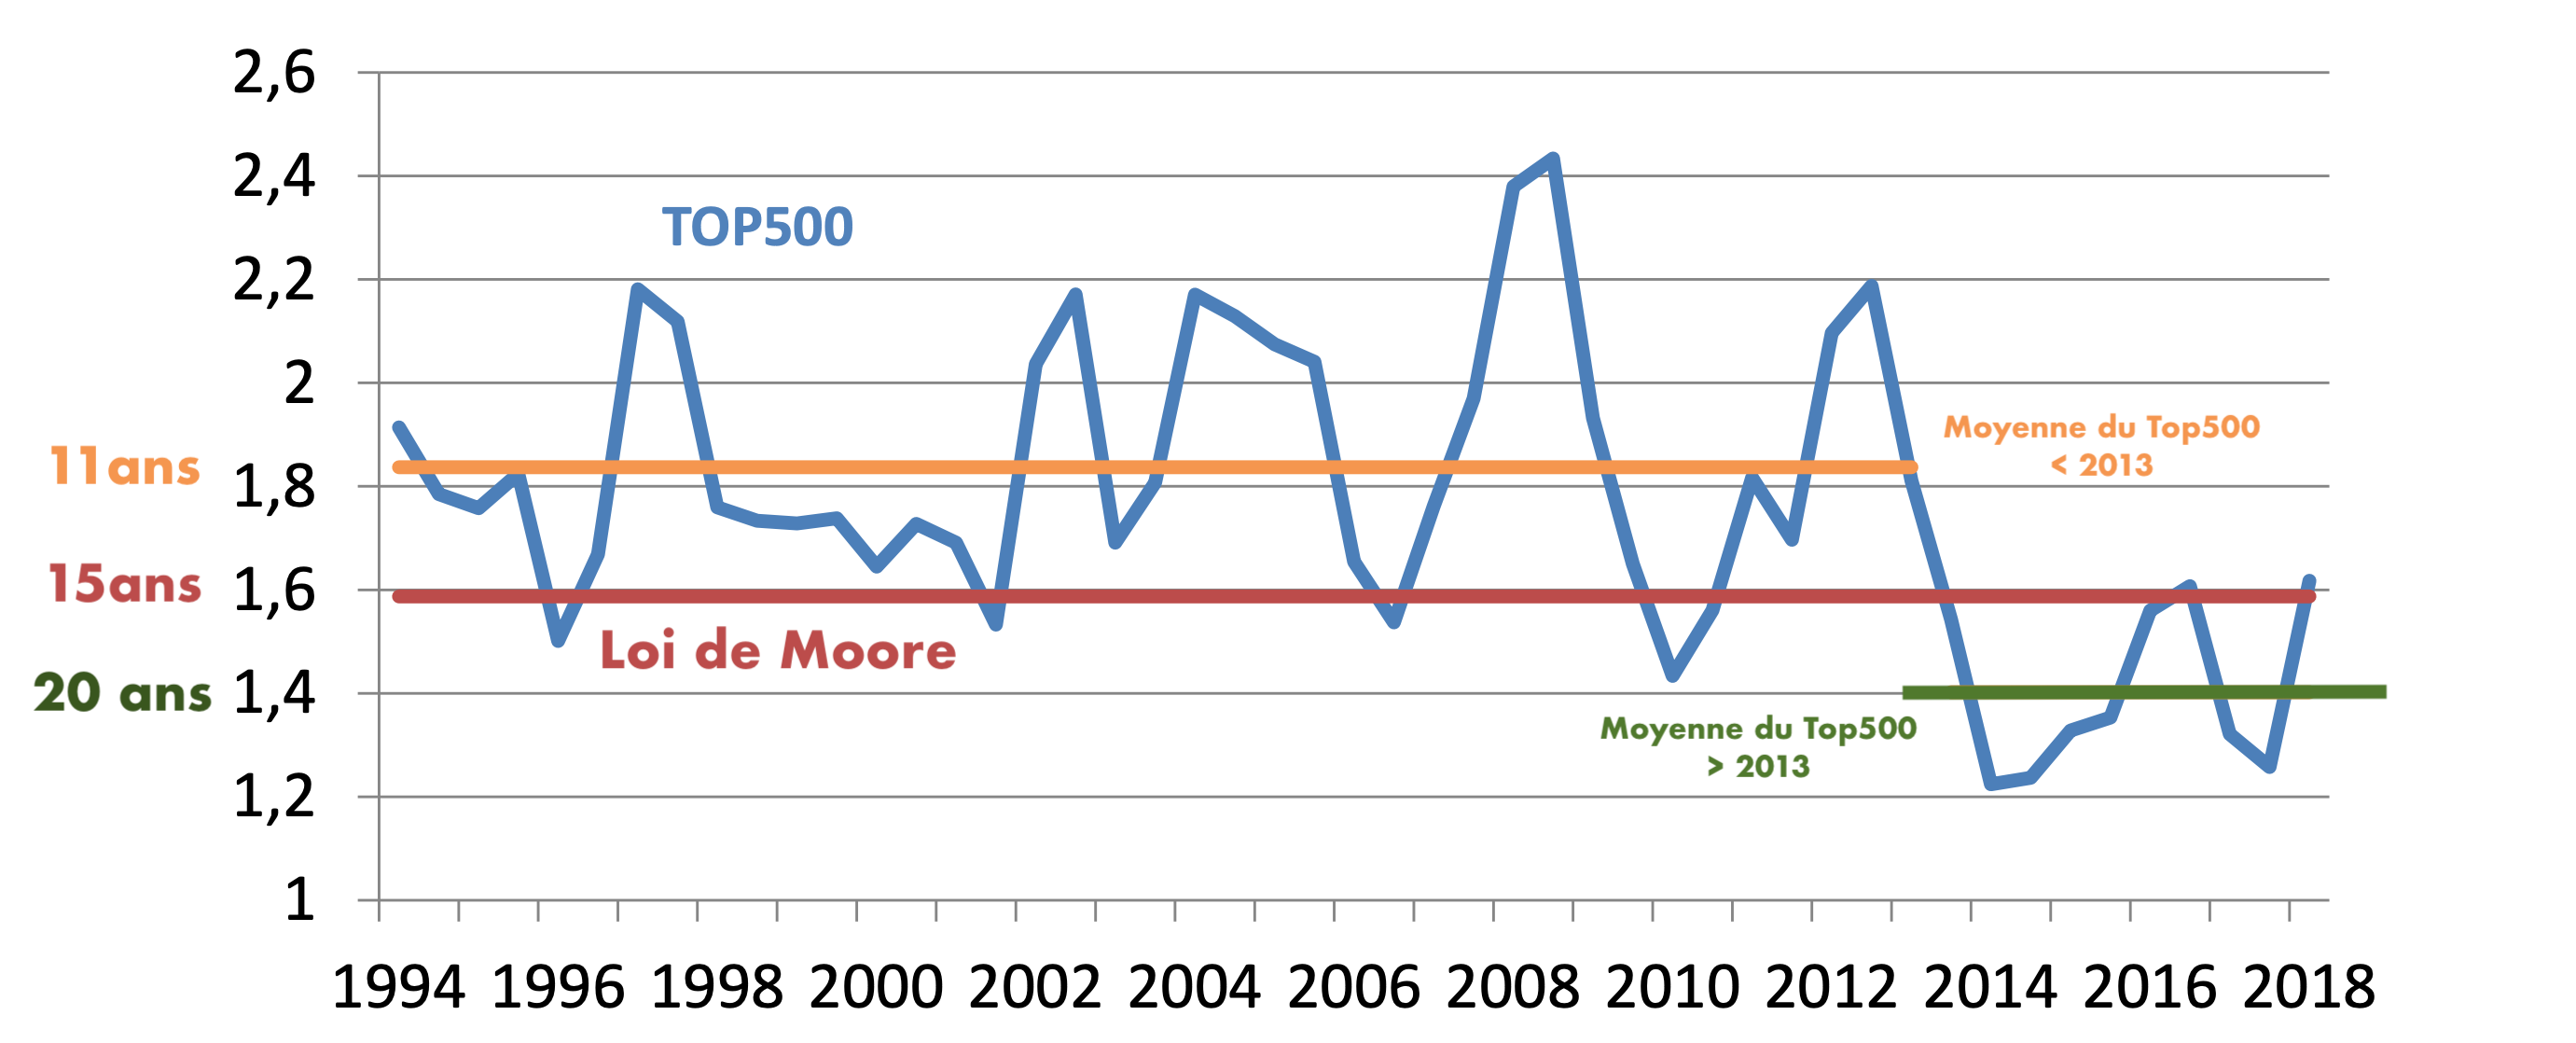
\includegraphics[width=12cm]{images/moore_vs_top500.png}
                \caption{\label{fig:moore_vs_top500} Évolution annuelle des performances du Top500\protect\footnotemark}
                    \end{figure}
                \footnotetext{Graphique insipiré de la présentation du Top500 lors de la conférence ISC18 - \textit{Highlights of the 51st TOP500 List}}
        
                
                Dans la \autoref{sec:denard}, nous avons discuté de l'augmentation de la fréquence des processeurs et introduit \textbf{la loi de Dennard} \cite{Dennard1974}. Ces équations ont assuré l'augmentation de la fréquence des processeurs, de 40\% tous les 2 ans pendant plus de trente ans. À cause des courant de fuites \cite{Wulf1995}. augmentant exponentiellement avec la finesse de gravure des transistors, la consommation électrique des processeurs a elle aussi augmentée. Dans la \autoref{sec:denard}, nous expliquons comment la réduction de la taille des transistors et l'augmentation de la fréquence des processeurs augmentent la consommation électrique de circuit. L'énergie utilisé par le processeur étant dissipée sous forme de chaleur, il est devenue très difficile de refroidir ces architectures. Le refroidissement nécessitant aussi d'être alimenté électriquement. Cette limitation physique empêchant d'augmenter la puissance électrique des processeurs est appelé \textit{power wall} \cite{Kuroda2001}.
                
                Si l'utilisation de processeur multi-coeur a permis de continuer d'augmenter la performance des processeurs malgré la faible évolution des fréquence, l'ajout de coeur à lui aussi atteint ses limites. En effet, comme démontré dans la \autoref{sec:parallele_perf}, l'augmentation des niveaux de parallélisme atteint lui aussi ses limites lorsque les applications contiennent des zones de codes séquentiels. Même des applications comme le benchmark \verb|HPL| sont impacté par \textbf{la loi d'Amdahl}, et l'ajout de coeurs s'est révélé de moins en moins efficace. On remarque sur la \autoref{fig:evo_proc} que le nombre de coeurs a peu évolué ces dix dernières années.
        
        %%%%%%%%%%%%%%%%%%%%%%%%%%%%%%%%%%%%%%%%%%%%%%%%%%%%%%%%%%%%%%%%%%%%%%%%%%%% 
        \paragraph{Déséquilibre des microarchitectures.} Dans la \autoref{sec:memory_wall_gap}, nous avons étudié la disparité des évolutions technologiques reçu par les processeseurs et par les mémoires. Cet écart à évolué au fil des années et il est aujourd'hui appelé \textit{mur de la mémoire} \cite{Rojas1997}  (\textit{memory wall} ou encore \textit{memory gap}). Si on regarde l'évolution des performances des différentes parties du système on peut constater de réelles différences:
            \begin{itemize}
                \item Les performances calculatoires des processeurs (le nombre d'opération flotantes réalisables par cycle) à \textbf{augmenté de 50\%} en moyenne par an.
                \item La bande passante entre le processeur et la mémoire à augmenté de 23\% par an
                \item La latence des requêtes mémoire a \textbf{diminué de 4\% }par an
                \item La bande passante sur le réseau à \textbf{augmenté de 20\%} par an
            \end{itemize}
        La \autoref{pic:cpuvsmemory} montre le déséquilibre entre ces deux parties fondamentales des architectures Von Neumann. Ce déséquilibre empêche aujourd'hui le système mémoire de transférer les données suffisament rapidement pour que la totalité des unités de calculs soient constamment actives. Pourtant, 50\% des broches d'un processeur récent sont allouées au système mémoire. Une large parties des applications HPC est limitées par la performance du système mémoire. Ainsi, bien que les performances de calculs des processeurs s'améliorent, ces applications ne peuvent pas en bénéficier. La plupart des supercalculateurs atteignent rarement une efficacité de 80\% sur une application simple comme Linpack \cite{Dongarra2003}. Pour des applications réelles, cette efficacité est encore plus faible, parfois inférieure à 10\% \cite{Oliker2005}.
            
                
        \begin{figure}
        \center
        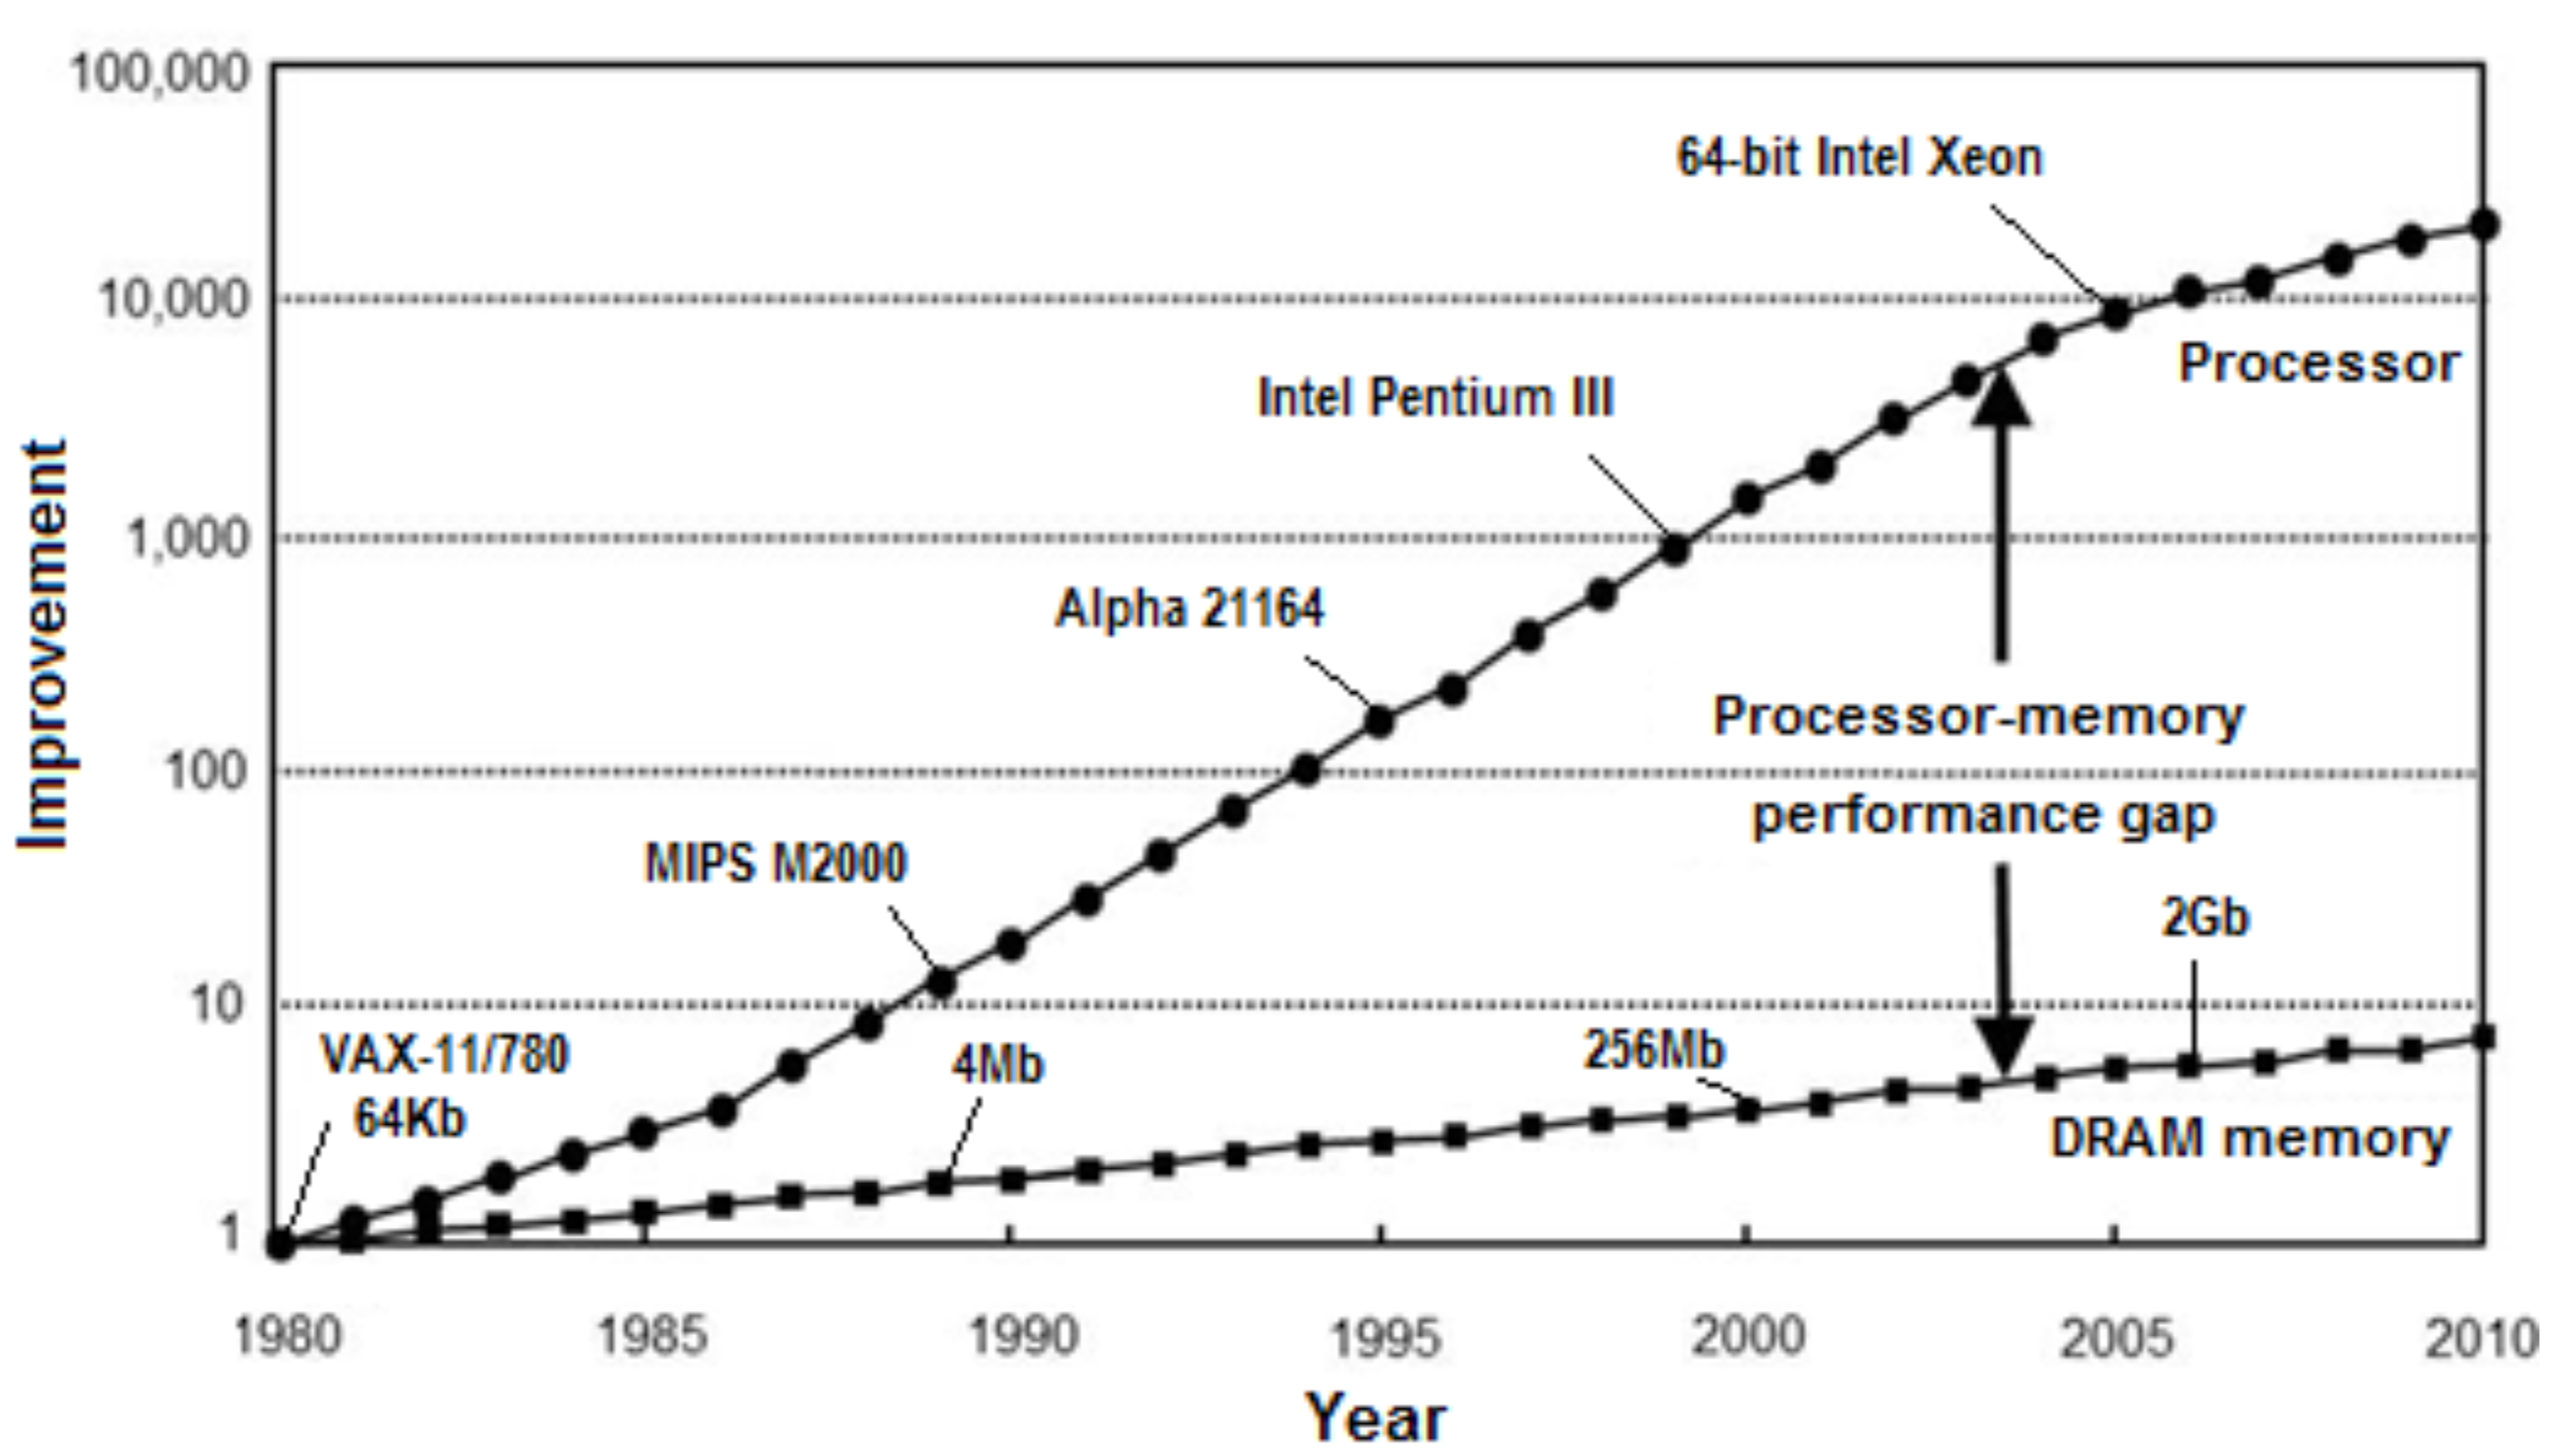
\includegraphics[width=10cm]{images/cpu_cpu_vs_memory.png}
        \caption{\label{pic:cpuvsmemory} Progression de la performance des processeurs et des mémoires. La performance de plusieurs générations de processeurs a été mesurée à l'aide du benchmark SPECint \cite{Efnusheva2017ASO}. La performance des mémoires est la mesure des latences d’accès mémoire (CAS et RAS) des mémoires DRAM.}
        \end{figure}
                
             
    
        %%%%%%%%%%%%%%%%%%%%%%%%%%%%%%%%%%%%%%%%%%%%%%%%%%%%%%%%%%%%%%%%%%%%%%%%%%%% 
        \paragraph{Les centres de données.} Divers facteurs rendent difficiles la constructions de supercalculateurs plus gros et plus puissant. Les deux principaux étant l'énergie et l'économie. Le première limite physique rencontrée par les clients de HPC est l'enveloppe énergétique disponible. Ajouter des serveurs pour la construction d'un supercalculateur plus puissant nécessite une plus grande puissance élèctrique. Cependant, les sites ou sont construit ces centre de données, ont des alimentations déjà existante et qui ne peuvent pas supporter de plus grandes puissances. Une partie des utilisateurs sont donc limités par cette enveloppe énergétique et doivent l'utiliser le plus efficacement pour la transformer en puissance de calcul. Les applications étant de plus en plus tournée sur l'utilisation de grand jeu de données, la consommation des applications n'en est qu'augmentée \cite{Kothe2016}. En effet, la coût du transfert d'une ligne de cache de la mémoire au processeur est supérieur de plusieurs facteur au coût d'une opération sur celle-ci (voir \autoref{fig:energy_pj}).
        
        \begin{figure}
        \center
        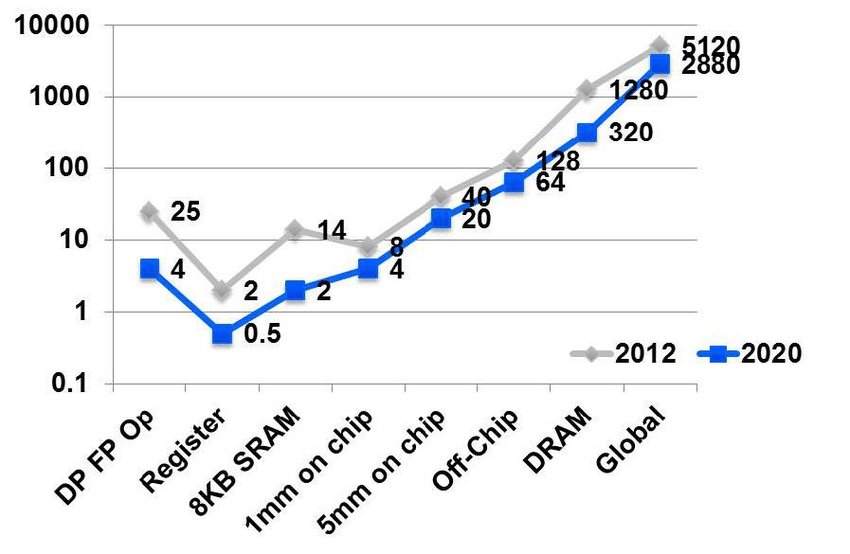
\includegraphics[width=10cm]{images/energy_pj.png}
        \caption{\label{fig:energy_pj} Coût énergétique, en picojoules (pJ) par opération à virgule flottante de 64 bits, pour diverses opérations courantes dans un ordinateur. La ligne supérieure (grise) caractérise les estimations des coûts de l'énergie en 2012 pour la technologie, et la ligne inférieure (bleue) prévoit les coûts en 2020 \cite{Leland2014}.}
        \end{figure}
        
        
        \paragraph{Économie.} Le prix des supercalculateurs est un frein à la construction de centre toujours plus puissant. On peut s'en apercevoir en regardant l'a différence d'évolution de performance du dernier supercalculateur du Top500 (voir \autoref{fig:Top500_Poor}). Le décrochage des performances du Top500, autour de 2012, étudié dans la section précédente, intervient plus de 4 ans après le décrochage du dernier du classement (en 2008). De plus, on peut étudier la répartition de la performances du Top500 entre les supercalculateurs. En 2004, il fallait agréger les 80 premiers supercalculateurs du classement pour obtenir la moitié de la performance cumulée du Top500. En 2019, il faut seulement cumuler la puissance des 28 premiers. Ceci montre que les plateformes en haut du classement ont tendances à évoluer plus vite que celle du bas. Les calculateurs les moins puissant du classement sont généralement ceux avec les plus petits budgets. Grâce à l'analyse du Top500, nous pouvons estimer que l'économie est un des freins participant au ralentissement de l'évolution des performances des architectures.
        
        
        \begin{figure}
        \center
        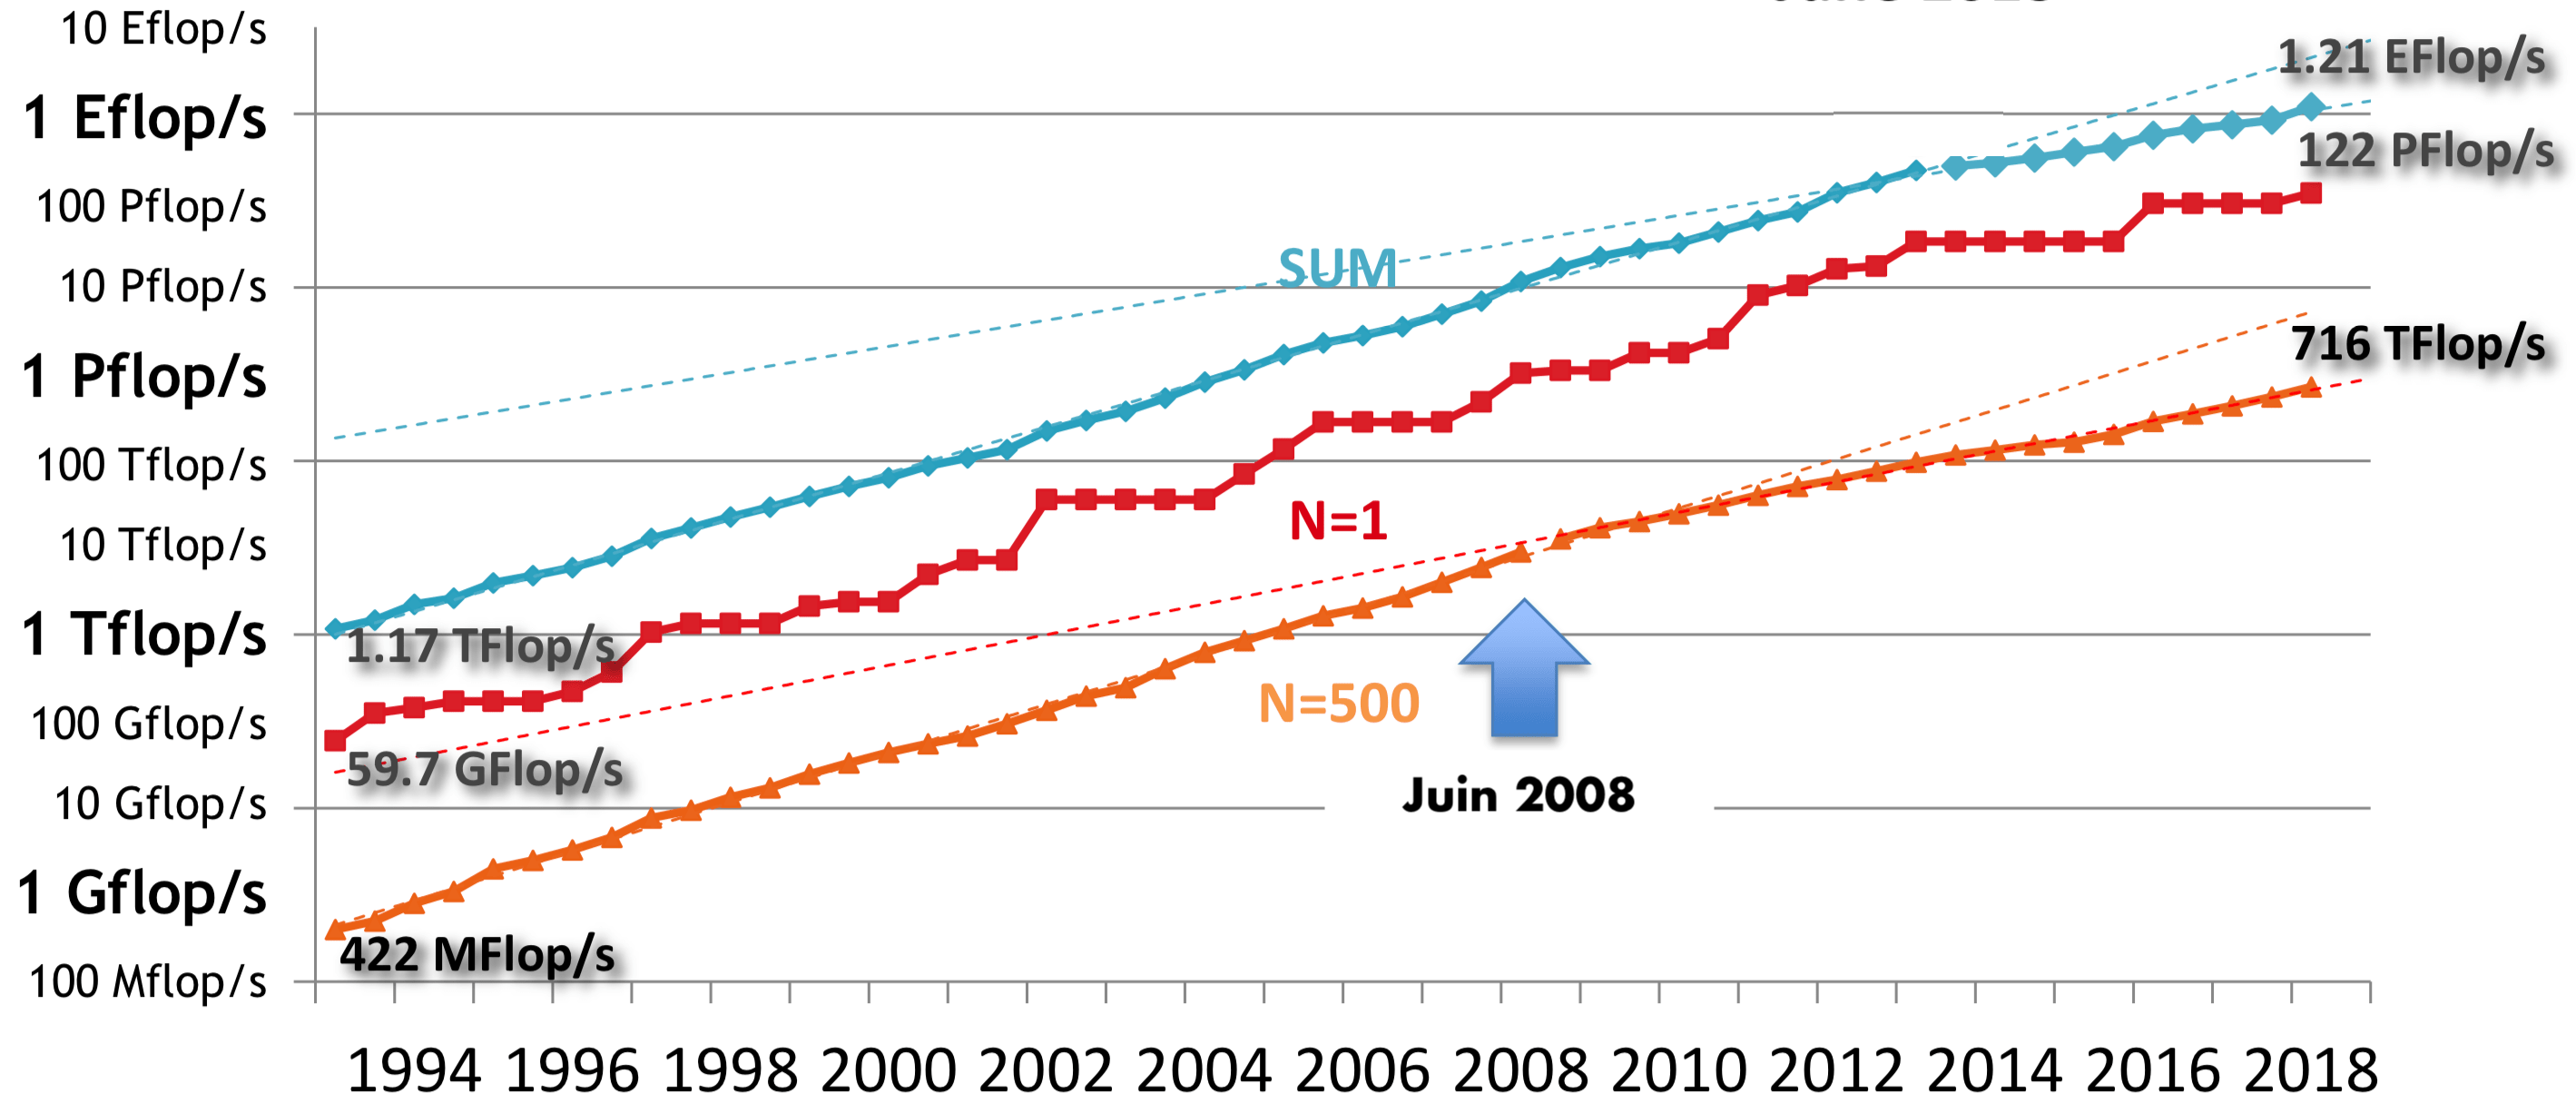
\includegraphics[width=14cm]{images/Top500_Poor.png}
        \caption{\label{fig:Top500_Poor} Évolution des performances du Top500: la puissance cumulée (en bleu), le premier (en rouge) et le dernier (en orange)\protect\footnotemark}
        \end{figure}
        \footnotetext{Graphique tiré de \url{https://www.top500.org/news/112019-highlights/}}
      